% SC4002 --- Chapter 4: Sequence Labeling --- HMM, CRF, BiLSTM-CRF (0->100 ground-up)
\chapter{Sequence Labeling: HMM, CRF, and BiLSTM-CRF}
\label{ch:sequence}

\begin{quote}
\emph{``A word in isolation is ambiguous; a word in context is a decision.''} --- This chapter turns tagging into a structured prediction problem where labels depend on each other.
\end{quote}

\noindent\fbox{\parbox{\dimexpr\linewidth-2\fboxsep-2\fboxrule}{%
\textbf{From zero: no sequence background assumed.} We start from the everyday idea of \emph{labeling each word} (is it a noun? a person name?) and ask why independent classifiers fail. Then we formalize dependencies via HMMs, fix their bias with CRFs, and finally learn features with BiLSTM-CRF. Every formula is motivated by a picture first.}}
\vspace{0.4em}

\section*{Learning Outcomes}
After this chapter you will be able to:
\begin{enumerate}[label=(L\arabic*)]
    \item frame POS tagging and NER as sequence labeling and explain why label dependencies matter;
    \item define HMM parameters (transition, emission) and decode with the Viterbi algorithm;
    \item contrast locally normalized MEMMs with globally normalized CRFs and write the CRF objective;
    \item describe the BiLSTM-CRF architecture and why it combines representation learning with structured decoding;
    \item implement Viterbi decoding and apply it to a tagging example.
\end{enumerate}

% ============================================================
\section{Tagging as Labeling: Why Context Matters}
\label{sec:tagging-intuition}
\paragraph{Intuition.} Read ``\emph{Time flies like an arrow.}'' Is \emph{flies} a verb or noun? In ``\emph{fruit flies}'' it is a noun. The same word gets different tags depending on neighbours. Sequence labeling assigns a label $y_t$ to each token $x_t$ in $\mathbf{x}=(x_1,\dots,x_T)$, producing $\mathbf{y}=(y_1,\dots,y_T)$. Two canonical tasks: \emph{POS tagging} (labels like \textsc{Noun}, \textsc{Verb}, \textsc{Adj}) and \emph{NER} (labels like \textsc{B-Per}, \textsc{I-Per}, \textsc{B-Loc}, \textsc{O} with BIO scheme).

\paragraph{Why not classify each position independently?} An independent classifier predicts $y_t$ from $x_t$ alone, ignoring that tags have grammar: determiners precede nouns, \textsc{I-Per} cannot follow \textsc{O} without \textsc{B-Per}. Dependencies are constraints. If we predict $\hat{y}_t=\arg\max_y P(y\mid x_t)$ per position, we may output invalid sequences (e.g., \textsc{B-Per} followed by \textsc{I-Loc}). Structured models score \emph{entire sequences} jointly, trading local confidence for global coherence.

\paragraph{Example.} Sentence: ``\emph{Alice visited Paris}'' $\to$ NER tags \textsc{B-Per}, \textsc{O}, \textsc{B-Loc}. Knowing $y_1=\textsc{B-Per}$ makes $y_2=\textsc{O}$ more likely than \textsc{I-Per}, because a person name rarely continues with a verb. The model must learn transition preferences $P(y_t\mid y_{t-1})$ alongside word evidence.

% ============================================================
\section{Hidden Markov Models and the Viterbi Algorithm}
\label{sec:hmm}
\paragraph{Intuition.} Imagine hidden weather (Sunny/Rainy) generating what you observe (walk/shop/clean). You see the actions, not the weather. An HMM assumes hidden states $y_t$ evolve as a Markov chain and each emits an observation $x_t$.

\paragraph{Formal definition.} An HMM defines $K$ hidden states and vocabulary $V$:
\begin{align}
    A_{ij} &= P(y_t=j \mid y_{t-1}=i) &&\text{transition, } K\times K \label{eq:trans}\\
    B_{j}(w) &= P(x_t=w \mid y_t=j) &&\text{emission, } K\times V \label{eq:emit}\\
    \pi_j &= P(y_1=j) &&\text{initial distribution.} \nonumber
\end{align}
The joint probability of a state--observation pair factorizes:
\begin{equation}
P(\mathbf{y},\mathbf{x}) = \pi_{y_1} B_{y_1}(x_1)\prod_{t=2}^{T} A_{y_{t-1},y_t}\,B_{y_t}(x_t).
\label{eq:hmm-joint}
\end{equation}
Learning estimates $A,B,\pi$ by counting (MLE) or EM (Baum-Welch) when states are unobserved.

\paragraph{Decoding: Viterbi.} At test time we want $\mathbf{y}^*=\arg\max_{\mathbf{y}} P(\mathbf{y}\mid\mathbf{x})\propto P(\mathbf{y},\mathbf{x})$. The trellis has $K\times T$ nodes; Viterbi is dynamic programming:
\begin{equation}
\delta_t(j)=\max_{y_{1:t-1}} P(y_{1:t-1}, y_t=j, x_{1:t}),\quad
\delta_t(j)=\max_i\big[\delta_{t-1}(i)\,A_{ij}\big]\cdot B_j(x_t),
\label{eq:viterbi}
\end{equation}
with backpointers $\psi_t(j)=\arg\max_i \delta_{t-1}(i)A_{ij}$. Complexity $O(TK^2)$, linear in length. Fig.~\ref{fig:hmm-trellis} visualizes the trellis.

\begin{figure}[h]
\centering
\begin{tikzpicture}[
  stnode/.style={circle, draw=blue!60!black, thick, fill=blue!15, minimum size=7mm, font=\scriptsize},
  obsnode/.style={rectangle, draw=green!55!black, thick, fill=green!15, rounded corners=2pt, minimum size=6mm, font=\scriptsize},
  arr/.style={-{Latex[length=2.2mm]}, thick, color=blue!50!black},
  emarr/.style={-{Latex[length=2mm]}, thick, dashed, color=green!50!black}
]
% time cols
\foreach \t in {1,2,3,4} {
  \node[font=\tiny, color=gray!70!black] at (\t*2.2,2.2) {$t{=}\t$};
}
% state rows: N and V for POS example
\foreach \t in {1,2,3,4} {
  \node[stnode] (s1\t) at (\t*2.2,1.2) {N};
  \node[stnode, fill=orange!15, draw=orange!60!black] (s2\t) at (\t*2.2,0.2) {V};
  \node[obsnode] (o\t) at (\t*2.2,-0.9) {$x_{\t}$};
  \draw[emarr] (s1\t) -- (o\t); \draw[emarr] (s2\t) -- (o\t);
}
% trellis edges (all-to-all)
\foreach \t in {1,2,3} {
  \pgfmathtruncatemacro{\nt}{\t+1}
  \draw[arr, color=blue!40!black] (s1\t) -- (s1\nt);
  \draw[arr, color=orange!60!black] (s1\t) -- (s2\nt);
  \draw[arr, color=orange!60!black] (s2\t) -- (s1\nt);
  \draw[arr, color=blue!60!black] (s2\t) -- (s2\nt);
}
% highlight best path
\draw[arr, ultra thick, color=red!70!black, opacity=0.85] (s11) -- (s22) -- (s23) -- (s14);
\node[font=\tiny, fill=red!8, rounded corners=2pt, inner sep=2pt] at (5.5,-1.7) {\textcolor{red!70!black}{bold = Viterbi best path}};
\node[font=\tiny, fill=yellow!8, draw=gray!40, rounded corners=2pt, inner sep=3pt] at (4.4,2.7) {\textcolor{blue!60!black}{$\blacksquare$ tag states} \ \textcolor{green!55!black}{$\blacksquare$ observations} \ \textcolor{orange!60!black}{$\blacksquare$ transitions}};
\end{tikzpicture}
\caption{HMM trellis for POS tagging ($K=2$: N/V). Circles are hidden tags, squares are words $x_t$, dashed arrows are emissions $B_j(x_t)$, solid arrows are transitions $A_{ij}$. Viterbi finds the maximum-weight path left-to-right.}
\label{fig:hmm-trellis}
\end{figure}

HMMs are generative: they model $P(\mathbf{x},\mathbf{y})$. This wastes capacity on $P(\mathbf{x})$ and forces strong independence assumptions (emission depends only on current tag). Discriminative successors avoid this.

% ============================================================
\section{Conditional Random Fields: Global Normalization}
\label{sec:crf}
\paragraph{Intuition.} A Maximum Entropy Markov Model normalizes locally at each position: $\sum_{y_t} P(y_t\mid y_{t-1}, \mathbf{x})=1$. If a state has only one outgoing transition, it always passes probability $1$ regardless of the observation---\emph{label bias}. Picture a narrow corridor: all flow is forced through it even if the wall evidence says stop.

\paragraph{Formal definition.} A linear-chain CRF models $P(\mathbf{y}\mid\mathbf{x})$ directly with global normalization:
\begin{equation}
P(\mathbf{y}\mid\mathbf{x}) = \frac{1}{Z(\mathbf{x})}\exp\!\Big(\sum_{t=1}^{T}\sum_{k=1}^{K}\lambda_k f_k(y_{t-1}, y_t, \mathbf{x}, t)\Big),
\label{eq:crf}
\end{equation}
where $f_k$ are feature functions (e.g., $f=\mathbf{1}\{y_t=\textsc{B-Per}, x_t=\text{``Alice''}\}$ or $f=\mathbf{1}\{y_{t-1}=\textsc{B-Per}, y_t=\textsc{I-Per}\}$), $\lambda_k$ are learned weights, and partition function
\begin{equation}
Z(\mathbf{x})=\sum_{\mathbf{y}'}\exp\big(\sum_{t,k}\lambda_k f_k(y'_{t-1},y'_t,\mathbf{x},t)\big)
\label{eq:partition}
\end{equation}
sums over \emph{all} $K^T$ label sequences---normalized once globally, not per step. This eliminates label bias: a path with weak observation support gets low global score even if local transitions are forced.

\paragraph{Training and inference.} Log-likelihood $\sum_i \log P(\mathbf{y}^{(i)}\mid\mathbf{x}^{(i)})$ is concave; gradients require $Z(\mathbf{x})$ and marginals computed by forward-backward (same $O(TK^2)$). Decoding again uses Viterbi on the score $\sum_{t,k}\lambda_k f_k$. Fig.~\ref{fig:crf-factor} shows the factor graph: factors couple adjacent labels and the whole observation.

\begin{figure}[h]
\centering
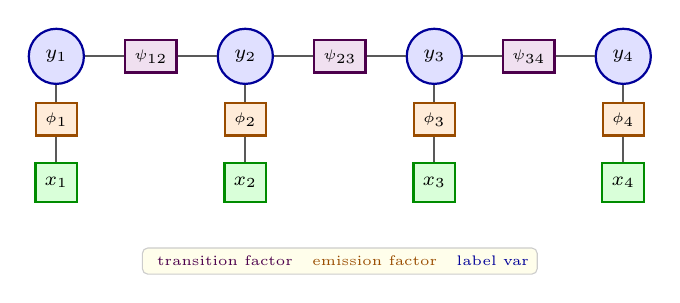
\begin{tikzpicture}[
  var/.style={circle, draw=blue!60!black, thick, fill=blue!12, minimum size=7mm, font=\scriptsize},
  obs/.style={rectangle, draw=green!55!black, thick, fill=green!15, minimum size=5mm, font=\scriptsize},
  fac/.style={rectangle, draw=violet!60!black, thick, fill=violet!12, minimum size=4mm, font=\tiny},
  edge/.style={thick, color=gray!70!black}
]
\node[var] (y1) at (0,1.0) {$y_1$}; \node[var] (y2) at (2.4,1.0) {$y_2$}; \node[var] (y3) at (4.8,1.0) {$y_3$}; \node[var] (y4) at (7.2,1.0) {$y_4$};
\node[obs] (x1) at (0,-0.6) {$x_1$}; \node[obs] (x2) at (2.4,-0.6) {$x_2$}; \node[obs] (x3) at (4.8,-0.6) {$x_3$}; \node[obs] (x4) at (7.2,-0.6) {$x_4$};
% transition factors
\node[fac] (f12) at (1.2,1.0) {$\psi_{12}$}; \node[fac] (f23) at (3.6,1.0) {$\psi_{23}$}; \node[fac] (f34) at (6.0,1.0) {$\psi_{34}$};
% emission factors
\node[fac, fill=orange!15, draw=orange!60!black] (e1) at (0,0.2) {$\phi_1$}; \node[fac, fill=orange!15, draw=orange!60!black] (e2) at (2.4,0.2) {$\phi_2$}; \node[fac, fill=orange!15, draw=orange!60!black] (e3) at (4.8,0.2) {$\phi_3$}; \node[fac, fill=orange!15, draw=orange!60!black] (e4) at (7.2,0.2) {$\phi_4$};
\draw[edge] (y1)--(f12)--(y2)--(f23)--(y3)--(f34)--(y4);
\foreach \i in {1,2,3,4} {\draw[edge] (y\i)--(e\i)--(x\i);}
\node[font=\tiny, fill=yellow!8, draw=gray!40, rounded corners=2pt, inner sep=3pt] at (3.6,-1.6) {\textcolor{violet!60!black}{$\blacksquare$ transition factor} \ \textcolor{orange!60!black}{$\blacksquare$ emission factor} \ \textcolor{blue!60!black}{$\blacksquare$ label var}};
\end{tikzpicture}
\caption{Linear-chain CRF factor graph. Variables $y_t$ (blue) connect via pairwise factors $\psi(y_{t-1},y_t,\mathbf{x})$ (violet) and unary factors $\phi(y_t,\mathbf{x})$ (orange) to observations $x_t$ (green). Global $Z(\mathbf{x})$ couples all factors.}
\label{fig:crf-factor}
\end{figure}

% ============================================================
\section{BiLSTM-CRF: Learning Features End-to-End}
\label{sec:bilstm-crf}
\paragraph{Intuition.} CRFs need hand-crafted features $f_k$. A BiLSTM learns them: read the sentence left-to-right and right-to-left, so each position sees full context, then let the CRF enforce tag grammar on top.

\paragraph{Architecture.} For token $x_t$, embed $\mathbf{e}_t$, run forward LSTM $\overrightarrow{\mathbf{h}}_t$ and backward LSTM $\overleftarrow{\mathbf{h}}_t$, concatenate $\mathbf{h}_t=[\overrightarrow{\mathbf{h}}_t;\overleftarrow{\mathbf{h}}_t]$. A linear layer maps $\mathbf{h}_t$ to emission scores $\mathbf{p}_t\in\mathbb{R}^K$ (one per tag). A learned transition matrix $\mathbf{T}\in\mathbb{R}^{K\times K}$ scores $T_{y_{t-1},y_t}$. Total sequence score:
\begin{equation}
s(\mathbf{x},\mathbf{y})=\sum_{t=1}^{T}\big(p_{t,y_t}+T_{y_{t-1},y_t}\big),\quad P(\mathbf{y}\mid\mathbf{x})=\frac{\exp s(\mathbf{x},\mathbf{y})}{\sum_{\mathbf{y}'}\exp s(\mathbf{x},\mathbf{y}')}.
\label{eq:bilstm-crf-score}
\end{equation}
Training maximizes log-likelihood via forward-backward; decoding is Viterbi over $(\mathbf{p},\mathbf{T})$. Fig.~\ref{fig:bilstm-crf} sketches the stack.

\begin{figure}[h]
\centering
\begin{tikzpicture}[
  emb/.style={rectangle, draw=teal!60!black, thick, fill=teal!15, minimum width=1.3cm, minimum height=0.6cm, font=\scriptsize, rounded corners=2pt},
  bilstm/.style={rectangle, draw=blue!60!black, thick, fill=blue!14, minimum width=1.6cm, minimum height=0.7cm, font=\scriptsize, rounded corners=3pt},
  crfbox/.style={rectangle, draw=violet!60!black, thick, fill=violet!12, minimum width=7.2cm, minimum height=0.75cm, font=\scriptsize, rounded corners=3pt},
  score/.style={rectangle, draw=orange!60!black, thick, fill=orange!14, minimum width=1.3cm, minimum height=0.55cm, font=\tiny, rounded corners=2pt},
  arr/.style={-{Latex[length=2mm]}, thick, color=gray!70!black}
]
% embeddings
\node[emb] (e1) at (0,0) {$\mathbf{e}_1$}; \node[emb] (e2) at (2,0) {$\mathbf{e}_2$}; \node[emb] (e3) at (4,0) {$\mathbf{e}_3$}; \node[emb] (e4) at (6,0) {$\mathbf{e}_4$};
\node[font=\tiny, color=teal!60!black] at (3,-0.6) {embeddings};
% BiLSTM
\node[bilstm] (b1) at (0,1.2) {BiLSTM}; \node[bilstm] (b2) at (2,1.2) {BiLSTM}; \node[bilstm] (b3) at (4,1.2) {BiLSTM}; \node[bilstm] (b4) at (6,1.2) {BiLSTM};
\foreach \i in {1,2,3,4} \draw[arr] (e\i)--(b\i);
\draw[arr, color=blue!50!black] (b1)--(b2); \draw[arr, color=blue!50!black] (b2)--(b3); \draw[arr, color=blue!50!black] (b3)--(b4);
\draw[arr, color=blue!35!black, dashed] (b4)--(b3); \draw[arr, color=blue!35!black, dashed] (b3)--(b2); \draw[arr, color=blue!35!black, dashed] (b2)--(b1);
% emission scores
\node[score] (p1) at (0,2.4) {$p_{1}$}; \node[score] (p2) at (2,2.4) {$p_{2}$}; \node[score] (p3) at (4,2.4) {$p_{3}$}; \node[score] (p4) at (6,2.4) {$p_{4}$};
\foreach \i in {1,2,3,4} \draw[arr] (b\i)--(p\i);
% CRF layer
\node[crfbox] (crf) at (3,3.5) {CRF layer: transition $\mathbf{T}$ + Viterbi decoding};
\foreach \i in {1,2,3,4} \draw[arr, color=violet!60!black] (p\i)--(crf);
\node[font=\scriptsize, color=violet!60!black] at (3,4.15) {$\mathbf{y}^*=\arg\max_{\mathbf{y}} s(\mathbf{x},\mathbf{y})$};
\end{tikzpicture}
\caption{BiLSTM-CRF architecture. Embeddings $\to$ BiLSTM (forward solid, backward dashed) $\to$ per-tag emission scores $\mathbf{p}_t$ $\to$ CRF with transition matrix $\mathbf{T}$ and global Viterbi decoding. Colours separate representation (teal/blue) from structured inference (orange/violet).}
\label{fig:bilstm-crf}
\end{figure}

BiLSTM-CRF became the pre-Transformer workhorse for NER: BiLSTM captures long-range lexical context, CRF prevents illegal BIO transitions (e.g., \textsc{I-Per} without \textsc{B-Per}).

\begin{lstlisting}[language=Python, caption={Viterbi decoding for HMM/CRF: works for both $A\cdot B$ and $(\mathbf{p},\mathbf{T})$ scores.}, label={lst:viterbi}]
import numpy as np

def viterbi(emission, trans, init):
    """emission: T x K, trans: K x K, init: K. Returns best path."""
    T, K = emission.shape
    dp = np.zeros((T, K))       # best log-prob to reach (t,j)
    back = np.zeros((T, K), dtype=int)
    dp[0] = np.log(init + 1e-12) + np.log(emission[0] + 1e-12)
    for t in range(1, T):
        for j in range(K):
            scores = dp[t-1] + np.log(trans[:, j] + 1e-12)
            back[t, j] = np.argmax(scores)
            dp[t, j] = scores[back[t, j]] + np.log(emission[t, j] + 1e-12)
    # backtrack
    path = [int(np.argmax(dp[T-1]))]
    for t in range(T-1, 0, -1):
        path.append(int(back[t, path[-1]]))
    return list(reversed(path)), float(np.max(dp[T-1]))

# Toy POS: tags [N, V], sentence "flies like"
emit = np.array([[0.1, 0.8], [0.4, 0.6]])   # P(word|tag)
trans = np.array([[0.7, 0.3], [0.4, 0.6]])  # P(tag_t|tag_{t-1})
init = np.array([0.6, 0.4])
print(viterbi(emit, trans, init))  # e.g. [1, 1] = V V
\end{lstlisting}

% ============================================================
\section{Syntactic Parsing: Who Did What to Whom}
\label{sec:parsing}
\paragraph{Intuition.} Tagging labels each word, but meaning lives in structure: in ``\emph{Alice visited Paris}'' who visited whom? Parsing recovers the tree. Two views dominate. \textbf{Constituency} groups words into nested phrases ($S\to NP~VP$, $VP\to V~NP$): \emph{Alice} is an $NP$, \emph{visited Paris} a $VP$. \textbf{Dependency} instead draws directed arcs head$\to$dependent: \emph{visited} is the root, with \emph{Alice} as subject and \emph{Paris} as object. Constituency shows grouping, dependency shows relations; most downstream tasks (relation extraction, semantic roles) read off the dependency arcs.
\paragraph{How to parse: shift-reduce sketch.} A transition-based parser scans left to right with a stack and a buffer, repeating three actions: \textsc{Shift} (push the next word), \textsc{Left-Arc} / \textsc{Right-Arc} (attach the top two stack items with a labeled arc and pop one), until one root remains. A classifier predicts each action from $(\mathrm{stack},\mathrm{buffer})$ features (or BiLSTM encodings); greedy decoding runs in linear time, beam search regains accuracy. The chart-based alternative, CKY, is dynamic programming over spans ($O(n^3)$) -- Viterbi's cousin from \S\ref{sec:hmm}, but over tree cells instead of tag columns.
\paragraph{Worked tiny parse.} ``\emph{Alice visited Paris}'': \textsc{Shift} \emph{Alice}, \textsc{Shift} \emph{visited}, \textsc{Left-Arc} (visited$\xleftarrow{\mathrm{subj}}$Alice), \textsc{Shift} \emph{Paris}, \textsc{Right-Arc} (visited$\xrightarrow{\mathrm{obj}}$Paris). Fig.~\ref{fig:parse-tree} shows the constituency twin of the same sentence.
\begin{figure}[h]
\centering
\begin{tikzpicture}[font=\scriptsize, >=Stealth, scale=0.85, level distance=10mm, sibling distance=22mm, every node/.style={draw, rounded corners=2pt, align=center, inner sep=3pt}]
\node[fill=violet!14, draw=violet!60!black] {S}
child {node[fill=blue!14, draw=blue!60!black] {NP\\Alice}}
child {node[fill=orange!14, draw=orange!60!black] {VP}
child {node[fill=green!15, draw=green!55!black] {V\\visited}}
child {node[fill=blue!14, draw=blue!60!black] {NP\\Paris}}};
\end{tikzpicture}
\caption{Constituency parse of ``Alice visited Paris'': $S\to NP~VP$ with $VP\to V~NP$. Colours separate clause (violet), phrases (blue/orange), and head verb (green); the matching dependency tree is rooted at \emph{visited} with subject/object arcs.}
\label{fig:parse-tree}
\end{figure}

% ============================================================
\section{Chapter Notes}
HMMs were introduced by Baum and Petrie (1966); Viterbi (1967) gave the decoding algorithm. Lafferty, McCallum and Pereira (2001) defined CRFs to fix label bias in MEMMs. Huang, Xu and Yu (2015) popularized BiLSTM-CRF for sequence tagging, now often replaced by Transformer-CRF. For BIO details see CoNLL-2003 NER shared task.

% ============================================================
\section{Exercises}
\label{sec:ch04-exercises}
\begin{enumerate}[label=E4.\arabic*, leftmargin=*, itemsep=0.7em]
    \item \textbf{Independent vs.\ structured.} Give a 3-word sentence and a tag set of size 2 where per-position argmax yields a different sequence than joint argmax. Compute both predictions with concrete $P(y_t\mid x_t)$ and $A_{ij}$ to show the gap.
    \item \textbf{Viterbi by hand.} HMM with tags $\{\textsc{N},\textsc{V}\}$, $A=[(0.8,0.2),(0.3,0.7)]$, $B_{\textsc{N}}(\text{``flies''})=0.1$, $B_{\textsc{V}}(\text{``flies''})=0.6$, $\pi=(0.5,0.5)$. For $\mathbf{x}=(\text{``flies''},\text{``flies''})$, fill $\delta_t(j)$ and $\psi_t(j)$ tables and backtrack the best path. What is $P(\mathbf{y}^*,\mathbf{x})$?
    \item \textbf{Label bias.} Construct a 2-state MEMM where state $s_1$ has one outgoing edge and $s_2$ has two. Show that $P(y_t\mid y_{t-1}=s_1,\mathbf{x})=1$ regardless of $\mathbf{x}$, while a CRF with the same features can assign low probability to the forced path. Explain why global $Z(\mathbf{x})$ fixes this.
    \item \textbf{CRF feature design.} Write 5 feature functions $f_k(y_{t-1},y_t,\mathbf{x},t)$ useful for NER on ``Bank of America'': include one transition, one word-identity, one capitalization, one gazetteer, and one suffix feature. Give each a weight sign and justify.
    \item \textbf{BiLSTM-CRF extension.} Explain why emission scores $\mathbf{p}_t$ come from $\mathbf{h}_t=[\overrightarrow{\mathbf{h}}_t;\overleftarrow{\mathbf{h}}_t]$ rather than $\overrightarrow{\mathbf{h}}_t$ alone. Sketch how to replace BiLSTM with a Transformer encoder while keeping the CRF layer unchanged, and state which equations stay the same.
\end{enumerate}
% End of Chapter 4
